% !TEX TS-program = pdflatex
% !TEX encoding = UTF-8 Unicode

% This is a simple template for a LaTeX document using the "article" class.
% See "book", "report", "letter" for other types of document.

\documentclass[11pt]{article} % use larger type; default would be 10pt

\usepackage[utf8]{inputenc} % set input encoding (not needed with XeLaTeX)

%%% Examples of Article customizations
% These packages are optional, depending whether you want the features they provide.
% See the LaTeX Companion or other references for full information.

%%% PAGE DIMENSIONS
\usepackage{geometry} % to change the page dimensions
\geometry{a4paper} % or letterpaper (US) or a5paper or....
% \geometry{margin=2in} % for example, change the margins to 2 inches all round
% \geometry{landscape} % set up the page for landscape
%   read geometry.pdf for detailed page layout information

\usepackage{caption}
\usepackage{hyperref}

\usepackage{graphicx} % support the \includegraphics command and options

% \usepackage[parfill]{parskip} % Activate to begin paragraphs with an empty line rather than an indent

%%% PACKAGES
\usepackage{array} % for better arrays (eg matrices) in maths
\usepackage{paralist} % very flexible & customisable lists (eg. enumerate/itemize, etc.)
\usepackage{verbatim} % adds environment for commenting out blocks of text & for better verbatim
\usepackage{subfig} % make it possible to include more than one captioned figure/table in a single float
\usepackage{natbib} % nice citations
% These packages are all incorporated in the memoir class to one degree or another...



%%% HEADERS & FOOTERS
\usepackage{fancyhdr} % This should be set AFTER setting up the page geometry
\pagestyle{fancy} % options: empty , plain , fancy
\renewcommand{\headrulewidth}{0pt} % customise the layout...
\lhead{}\chead{}\rhead{}
\lfoot{}\cfoot{\thepage}\rfoot{}

%%% SECTION TITLE APPEARANCE
\usepackage{sectsty}
\allsectionsfont{\sffamily\mdseries\upshape} % (See the fntguide.pdf for font help)
% (This matches ConTeXt defaults)

%%% ToC (table of contents) APPEARANCE
\usepackage[nottoc,notlof,notlot]{tocbibind} % Put the bibliography in the ToC
\usepackage[titles,subfigure]{tocloft} % Alter the style of the Table of Contents
\renewcommand{\cftsecfont}{\rmfamily\mdseries\upshape}
\renewcommand{\cftsecpagefont}{\rmfamily\mdseries\upshape} % No bold!

%%% END Article customizations

%%% The "real" document content comes below...

\title{Procedurally grown trees}
\author{Andreas Valter}
%\date{} % Activate to display a given date or no date (if empty),
         % otherwise the current date is printed

\begin{document}
\maketitle
\section{Background}
When modelling the growth of trees, their growth follows a specific procedure that can be modelled.
The system is called a fractal and is a natural phenomenon where the same pattern repeats itself at different scales.
The smallest branch of a tree looks like a tree itself.
But even if a tree follows these rules, it will also take other things, like the amount of sun the leaves can absorb, water supply into consideration when deciding the fate of each branch and the whole tree.
This makes it so that when observing a real tree, the features of a fractal pattern is somewhat visible but it is hidden behind the fate of the tree as it has grown.
If these are taken into consideration when creating the fractal pattern of the tree, it will look close to a real tree.

When simulating the growth of a tree, it is important to define a couple terms that helps when describing the different steps of the growth procedure.
The point where leafs are attached to a stem are called \emph{nodes}.
The part of the stem between two nodes are called an \emph{inter-node}.
An inter-node, connected leafs and bud is a \emph{metamer}.
\ref{Palubicki}

\section{Implementation}
The model was implemented in C++ using OpenGL and GLSL for both computation and rendering.
It follows the report by \citet{Palubicki} that describes a method for creating self-organizing trees.
\citet{Palubicki} describes a general outline of the method they present, as well as several alternatives for the steps that makes up for the total algorithm.
Due to time constraints, all of the described methods has not been implemented in this report.

\subsection{Tree generation}


\subsubsection{Environmental input}
The presented method starts with environmental input where the environment around each existing bud is examined to determine the state for those parts of the tree.
\citet{Palubicki} presents two different techniques for handling the availability of growth in space around the tree and the optimal growth direction for branches.
One is called \emph{space colonization} and the other is called \emph{shadow propagation}.

Space colonization uses a uniform distribution of points in the world, each bud has an occupancy zone as well as a perception volume.
When evaluating available space, available points within the perception volume are found.
By summarizing the direction towards each of them, a optimal growth direction is found.
When adding new points, the points within the occupancy zone are consumed.
A binary shadow value is also provided that is zero when no points are available and one when points were found.

Shadow propagation uses a voxel grid to keep track of the environment around each bud.
Each newly formed bud adds a shadow value to the voxel grid in a pyramid below it with a shadow value that propagates to the voxels underneath.
This imitates a prenumbra shadow from each bud and as the shadow value increases, the probability for growth towards that specific voxel decreases.
Optimal directions are calculated by finding the gradient of the shadow grid in the bud point to make it grow towards the direction where there is the most light.
When bud points are not contained within the grid, the size of the grid is doubled in that direction until the resized grid covers the point.
The data from the previous grid are copied into the resized grid together with the data from the new bud point.

\subsubsection{Bud fate}
The technique that were implemented is an extension to the Borchet-Honda model that is described in \citet{Pablucki}.
The bud fate is decided using the shadow value retrieved from the environmental input calculation for each bud.
This value is then distributed towards the light accumalative producing the total light reached to each branch and its child branches.

The number of metamers produced by the bud is calculated as the light value floored and the length of the branch is the light value divided by the number of metamers.

\subsubsection{Shoots creation}
The bud fate decides what shoots to add and their length.
Metamers are added in an iterative fashion to the branches represented as a binary tree.
Each branch has two childs, the terminal and the lateral branch.

\subsubsection{Branch width}
The branch width is calculated by adding width back towards the root from the end branches of the tree.

This requires that shred branches are stored so that the width of the tree does not change in width as branches are removed.

\subsection{Rendering}
To be able to visualize the tree and to produce an output as quickly as possible, shaders were used to produce a model.
As the tree are done calculating the new state, the collection of branches are sent to the renderer.
The renderer converts the tree data to a buffer of packed data and uploads it to a compute shader.
The compute shader is responsible for converting the input data consisting of branch start points, end points and the width of the branch in each edge into quads.
The amount of quads generated gets decided by an input uniform.
The compute shader also calculates the normal and the texture coordinates for each branch.

The position of the faces belonging to each branch is calculated by extracting a vector that is perpendicular to the direction of the branch.
The second edge of the quad is calculated by rotating the position around the branch axis by an amount so that all of the quads covers the full 360 degrees.
Normals are received from the direction from the axis to each point.

Texture coordinates are calculated using three different LODs depending on the width of the branch.
The texture ID is stored together with the texture coordinate and to make sure that each branch receives an unique set of texture coordinates three atomic integers are used to give out positions in the texture map.
This causes a lot of texture space and allows for higher quality in the branches where it is useful.

The computed tree branches are then used to generate the texture map and a second shader pair consisting of a vertex shader and a fragment shader.
The vertex shader outputs the texture coordinates as positions but also sends the world position of each fragment.
These are then used as input to several noise functions that generates a diffuse map, normal map and displacement map of the tree bark.

The tree is rendered using a tessellation shader that use the displacement map to offset the generated vertices to their correct location.
The displacement can be scaled using a uniform.
The result is then drawn to the GBuffer using the diffuse and the normal texture to produce the final output.

Leafs are produced in a similar fashion using the position of the metamers and the branch directions.
The direction of the leafs are decided by weighing the gravity direction together with the branch direction to find the direction of the leaf.
This is done within a compute shader and results in a vertex buffer containing all leafs.
Leafs are created using simple geometry consisting of only two triangles.
The color is selected as different shades of green using the world position as lookup and a noise function to offset the value.

\section{Results}
When running the application, the growth of the tree is displayed in the application view port.
As the tree grows, leafs are dynamically added and moves as touched by a breeze.
\autoref{fig:res_1tree} shows a screen capture of a single tree grown over 20 growth cycles.

\begin{figure}[htp]
	\centering
	
\includegraphics[width=0.4\textwidth]{1tree.png}
	\caption{Single grown tree using the extended BH bud fate model.}
	\label{fig:res_1tree}
\end{figure}

The total time to grow the tree was 138ms and most of that time was spent adding points to the voxel grid.
This is visualized in \autoref{fig:res_timingTotal} where the total time per growth cycle is shown and divided into the required steps performed when generating the tree.

\begin{figure}[htp]
	\centering
	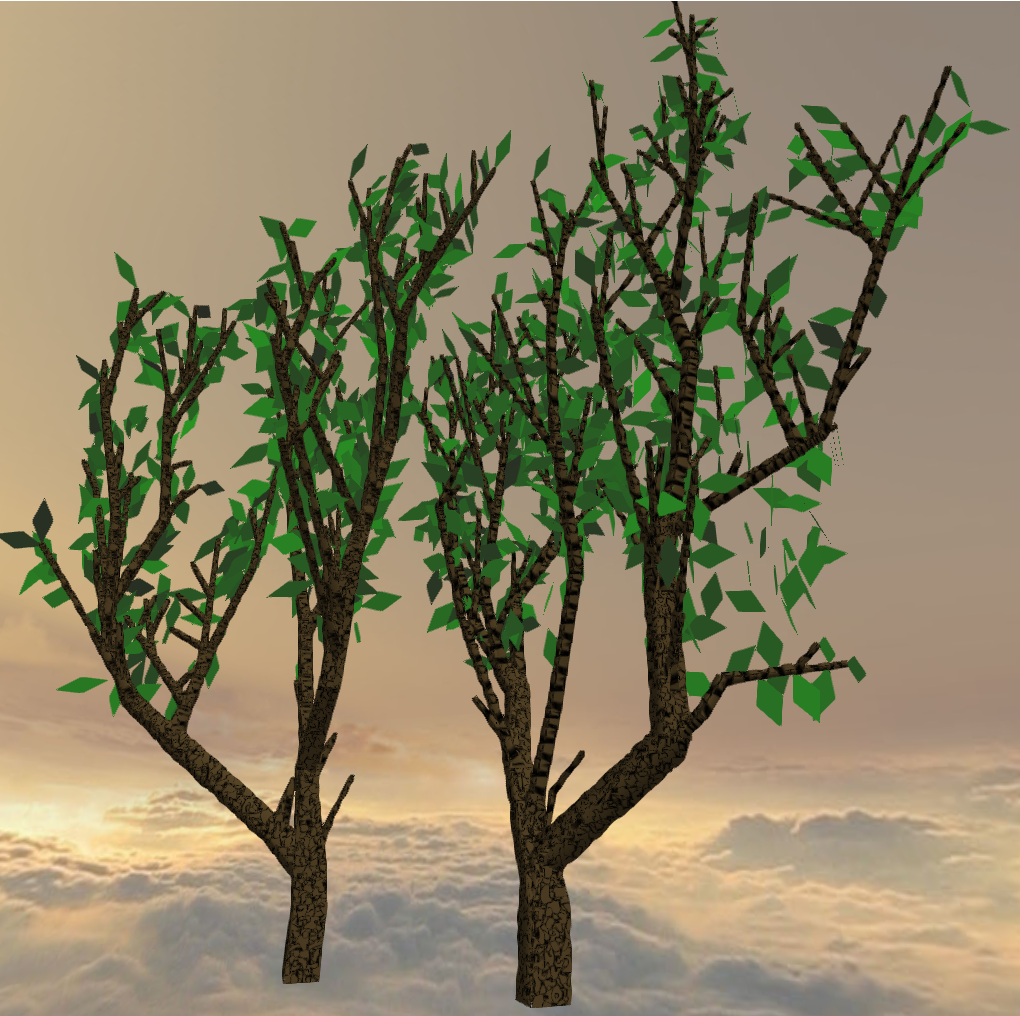
\includegraphics[width=0.4\textwidth]{2tree.png}
	\caption{Two grown tree using the extended BH bud fate model.}
	\label{fig:res_2tree}
\end{figure}

\autoref{fig:res_2tree} shows the same algorithm operating on two trees growing at the same time sharing grid.

\begin{figure}[htp]
	\centering
	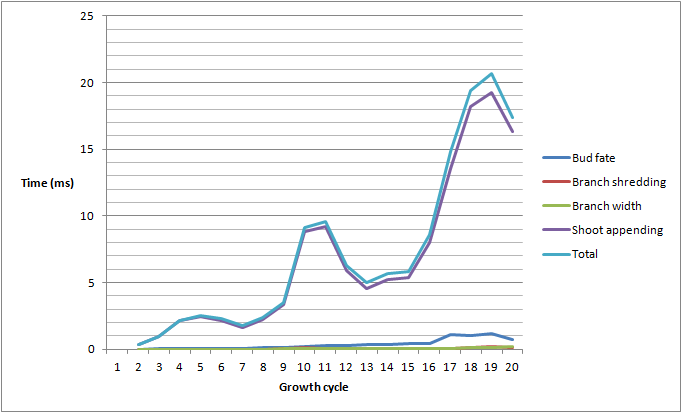
\includegraphics[width=0.8\textwidth]{timingTotal.png}
	\caption{Total simulation time per growth stage for a tree.}
	\label{fig:res_timingTotal}
\end{figure}

\begin{figure}[htp]
	\centering
	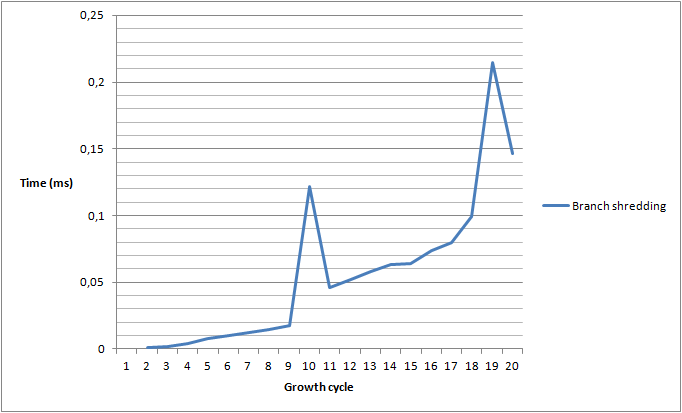
\includegraphics[width=0.8\textwidth]{timingBranchShred.png}
	\caption{Branch shredding on the .}
	\label{fig:res_timingTotal}
\end{figure}

\section{Conclusions}
The tree structure is thicker at the top part of the tree because of the shadow grid that shreds branches that shadowed by overlying branches.
That the extended BH model makes it almost impossible to create a main terminal branch in the tree pointing upwards.
This results in a lot wider trees that always has a branch at the begining.
By implementing the pirority bud fate model, the main branch could be prioritized, resulting in a tree more distinct tree shape with a thick terminal branch and smaller branches pointing out from it.

As can be seen in \autoref{fig:res_2tree}, the algorithm succesfully handles dynamic growth of several trees that interact with each other without intersections.

The speed of the tree generation could be increased using a octree structure for handling the grid, this would make it faster to increase the size of the grid while keeping the size of the grid smaller because it is a sparse structure that only keeps data for filled voxels.
And just as it is for real trees, computer generated trees are mostly air or empty voxels.

The quality of the textures could be increased by using a set of generated 2d textures for each branch and interpolate them between branches using weights in the joints.
Using several lods for the textures makes it possible to have a high quality of each tree while keeping them unique.
But they suffer from running out of texture space when the tree grows big enough.

\bibliographystyle{abbrv}
\bibliography{report}

\end{document}
